\documentclass[../main.tex]{subfiles}
\begin{document}
	
	\section{Avaliação 1}
		\begin{exercicio}{1}
			[1 ponto] Indique se as afirmações são verdadeiras ou falsas e justifique (o que vale a note é a justificativa):
			\begin{itemize}
				\item (V | F) A aplicação $\alpha(t)=(t^3,t^2)$, $t \in \mathbb{R}$ é uma curva regular.
				\item (V | F) Para curvas $\alpha \colon \mathbb{R}\to \mathbb{R}^2$ parametrizadas por comprimento de arco, os vetores $\alpha'(t)$ e $\alpha''(t)$ são ortogonais.
			\end{itemize}
		\end{exercicio}
		\begin{solucao}
			\begin{itemize}
				\item Falsa.
				\begin{align*}
					\alpha(t)=(t^3,t^2)
					&\Rightarrow \alpha'(t)=(3t^2,2t)\\
					&\Rightarrow \alpha'(0)=(0,0)
				\end{align*}
				Logo, como $\exists t\in \mathbb{R}, \alpha'(t)=(0,0)$, então $\alpha$ não é regular.
				\item Verdadeira.
				Note que, como $\alpha$ é parametrizada por comprimento de arco, $\|\alpha'(t)\|=1, \forall t \in \mathbb{R}$.
				Assim,
				\begin{align*}
					\|\alpha'(t)\|=1
					&\Rightarrow \langle \alpha'(t), \alpha'(t) \rangle =1\\
					&\Rightarrow (\langle \alpha'(t), \alpha'(t) \rangle)'=0\\
					&\Rightarrow \langle \alpha''(t), \alpha'(t) \rangle + \langle \alpha'(t), \alpha''(t) \rangle = 0\\
					&\Rightarrow \langle \alpha''(t), \alpha'(t) \rangle = 0\\
					&\Rightarrow \alpha''(t) \perp \alpha'(t)
				\end{align*}
				Logo, os vetores $\alpha'(t)$ e $\alpha''(t)$ são ortogonais $\forall t \in \mathbb{R}$.
			\end{itemize}
		\end{solucao}
		
		\begin{exercicio}{2}
			[1 ponto] Considere a curva
			\[
			\beta(s)=\bigg(\frac{(1+s)^{\tfrac{3}{2}}}{3},\frac{(1-s)^{\tfrac{3}{2}}}{3}, \frac{s}{\sqrt{2}}\bigg), -1<s<1
			\]
			\begin{enumerate}
				\item Provar que $\beta$ é parametrizada por comprimento de arco.
				\item Provar que $\tau=\kappa$
			\end{enumerate}
		\end{exercicio}
		\begin{solucao}
			\begin{enumerate}
				\item Devemos verificar que $\|\beta'(s)\|=1, \forall s\in (-1,1)$.
				\begin{align*}
					&\beta'(s)=\bigg(\frac{1}{3}\cdot \frac{3}{2}\cdot (1+s)^{\tfrac{1}{2}}\cdot (1),\frac{1}{3}\cdot \frac{3}{2}\cdot (1-s)^{\tfrac{1}{2}}\cdot (-1), \frac{1}{\sqrt{2}}\bigg)\\
					&\Rightarrow\beta'(s)=\bigg(\frac{(1+s)^{\tfrac{1}{2}}}{2},-\frac{(1-s)^{\tfrac{1}{2}}}{2}, \frac{1}{\sqrt{2}}\bigg)\\
					&\Rightarrow\|\beta'(s)\|=\bigg(\frac{(1+s)^{\tfrac{1}{2}}}{2}\bigg)^2+\bigg(-\frac{(1-s)^{\tfrac{1}{2}}}{2}\bigg)^2+ \bigg(\frac{1}{\sqrt{2}}\bigg)^2\\
					&\Rightarrow\|\beta'(s)\|=\bigg(\frac{1+s}{4}\bigg)+\bigg(\frac{1-s}{4}\bigg)+ \bigg(\frac{1}{2}\bigg)=1\\
				\end{align*}
				Assim, $\beta$ é parametrizada por comprimento de arco.
				\item Primeiro, vamos calcular $\beta'$, $\beta ''$, $\beta '''$ e $\beta'\wedge\beta''$.
				\begin{itemize}
					\item Como calculado em 2.1, $\beta'(s)=\bigg(\frac{(1+s)^{\tfrac{1}{2}}}{2},-\frac{(1-s)^{\tfrac{1}{2}}}{2}, \frac{1}{\sqrt{2}}\bigg)$
					\item $\beta''(s)=\bigg(\tfrac{1}{2}\cdot \frac{(1+s)^{-\tfrac{1}{2}}}{2}\cdot 1,-\tfrac{1}{2}\cdot \frac{(1-s)^{-\tfrac{1}{2}}}{2}\cdot (-1),0\bigg)=\bigg(\frac{1}{4(1+s)^{-1/2}},\frac{1}{4(1-s)^{1/2}},0\bigg)$
					\item $\beta'''(s)=\bigg(-\tfrac{1}{2}\cdot\frac{1}{4(1+s)^{3/2}},-\tfrac{1}{2}\cdot \frac{1}{4(1-s)^{3/2}}\cdot(-1),0\bigg)=\bigg(-\frac{1}{8(1+s)^{3/2}},\frac{1}{8(1-s)^{3/2}},0\bigg)$
					\item Segue o cálculo do produto vetorial entre $\beta'(s)$ e $\beta''(s)$
					
					\begin{align*}
						&\beta'(s)\wedge\beta''(s)\\
						&=\bigg(\det\begin{bmatrix} -\frac{(1-s)^{1/2}}{2} & \frac{1}{\sqrt{2}} \\ \frac{1}{4(1-s)^{1/2}} & 0 \end{bmatrix}, -\det\begin{bmatrix} \frac{(1+s)^{1/2}}{2} & \frac{1}{\sqrt{2}} \\ \frac{1}{4(1+s)^{1/2}} & 0 \end{bmatrix}, \det\begin{bmatrix} \frac{(1+s)^{1/2}}{2} & -\frac{(1-s)^{1/2}}{2} \\ \frac{1}{4(1+s)^{1/2}} & \frac{1}{4(1-s)^{1/2}} \end{bmatrix}\bigg)\\
						&=\bigg(-\frac{1}{4\sqrt{2}(1-s)^{1/2}}, \frac{1}{4\sqrt{2}(1+s)^{1/2}}, \frac{(1+s)^{1/2}}{8(1-s)^{1/2}}+\frac{(1-s)^{1/2}}{8(1+s)^{1/2}}\bigg)\\
						&=\bigg(-\frac{1}{4\sqrt{2}(1-s)^{1/2}}, \frac{1}{4\sqrt{2}(1+s)^{1/2}}, \frac{(1+s)+(1-s)}{8(1-s^2)^{1/2}}\bigg)\\
						&=\bigg(-\frac{1}{4\sqrt{2}(1-s)^{1/2}}, \frac{1}{4\sqrt{2}(1+s)^{1/2}}, \frac{1}{4(1-s^2)^{1/2}}\bigg)
					\end{align*}
				\end{itemize}
				A curvatura é dada por $\kappa_{\beta}(s)=\frac{\|\beta'(s)\wedge\beta''(s)\|}{\|\beta'(s)\|^3}$. No entanto, como provado em 2.1, $\|\beta'(s)\|=1$. Logo,
				\begin{align*}
					\kappa_{\beta}(s)
					&=\|\beta'(s)\wedge\beta''(s)\|\\
					&=\bigg(\frac{1}{32(1-s)}+\frac{1}{32(1+s)}+\frac{1}{16(1-s^2)}\bigg)^{\tfrac{1}{2}}\\
					&=\bigg(\frac{1+s+1-s+2}{32(1-s^2)}\bigg)^{\tfrac{1}{2}}\\
					&=\bigg(\frac{1}{8(1-s^2)}\bigg)^{\tfrac{1}{2}}=\frac{1}{2\sqrt{2}(1-s^2)^{1/2}}
				\end{align*}
				Calculando, agora, a torção, temos
				\begin{align*}
					&\tau_{\beta}(s)\\
					&=\frac{\langle\beta'(s)\wedge \beta''(s), \beta'''(s)\rangle}{\|\beta'(s)\wedge\beta''(s)\|^2}\\
					&=\bigg(\frac{1}{32\sqrt{2}(1-s)^{1/2}(1+s)^{3/2}}+\frac{1}{32\sqrt{2}(1+s)^{1/2}(1-s)^{3/2}}\bigg)\cdot \frac{1}{\|\beta'(s)\wedge\beta''(s)\|^2}\\
					&= \bigg(\frac{(1-s)+(1+s)}{32\sqrt{2}(1-s^2)^{3/2}}\bigg)\cdot\bigg(\frac{8(1-s^2)}{1}\bigg)=\bigg(\frac{2}{32\sqrt{2}(1-s^2)^{3/2}}\bigg)\cdot\bigg(\frac{8(1-s^2)}{1}\bigg)\\
					&=\frac{1}{2\sqrt{2}(1-s^2)^{1/2}}
				\end{align*}
				Portanto que
				$\begin{cases} \kappa_{\beta}(s)=\frac{1}{2\sqrt{2}(1-s^2)^{1/2}}\\ \tau_{\beta}(s)=\frac{1}{2\sqrt{2}(1-s^2)^{1/2}}\end{cases}\Rightarrow\kappa_{\beta}(s)=\tau_{\beta}(s)$
			\end{enumerate}
		\end{solucao}
		
		\begin{exercicio}{3}
			[1 ponto] Mostramos em sala que o vetor gradiente é ortogonal à tangente da curva de nível em um ponto dado. Esta questão visa exemplificar esse fato. Considere o campo escalar
			\[
			f(x,y)=(x^2+y^2)\ln(x^2+y^2)
			\]
			Defina a função campo gradiente de $f$. Escolha ao menos duas curvas de nível, defina a tangente à curva de nível. Calcule o gradiente do campo relativos às curvas escolhidas. Mostre que são ortogonais. Esboce as informações produzidas.
		\end{exercicio}
		\begin{solucao}
			Dada a função $f$, podemos calcular a função de seu campo gradiente.
			\begin{align*}
				\nabla f(x,y)
				&=\bigg(\frac{\partial f(x,y)}{\partial x}, \frac{\partial f(x,y)}{\partial y}\bigg)\\
				&=\bigg(\frac{\partial (x^2+y^2)\ln(x^2+y^2)}{\partial x}, \frac{\partial (x^2+y^2)\ln(x^2+y^2)}{\partial y}\bigg)\\
				&=\bigg(2x\ln(x^2+y^2)+(x^2+y^2)\frac{2x}{x^2+y^2}, 2y \ln(x^2+y^2)+(x^2+y^2)\frac{2y}{x^2+y^2}\bigg)\\
				&=\bigg(2x\big(1+\ln(x^2+y^2)\big), 2y\big(1+\ln(x^2+y^2)\big)\bigg)
			\end{align*}
			Agora, vamos de fato ao exemplo, com as duas curvas de nível escolhidas.
			\begin{enumerate}
				\item Primeira curva de nível escolhida: $f(x,y)=0$.
				\begin{align*}
					f(x,y)=0
					&\Rightarrow(x^2+y^2)\ln(x^2+y^2)=0\\
					&\Rightarrow \begin{cases}x^2+y^2=0\\ \ln(x^2+y^2)=0\Rightarrow x^2+y^2=1\end{cases}
				\end{align*}
				O primeiro caso é apenas um ponto, não tão interessante para a nossa análise. Peguemos, então, a curva $\gamma_1$ dada pela equação $x^2+y^2=1$, que pode ser parametrizada como $\gamma_1(t)=(\cos(t), \sin(t))\Rightarrow \gamma_1'(t)=(-\sin(t),\cos(t))$.
				
				Agora, considere $p$ um ponto arbitrário de $\gamma_1$.
				
				\begin{align*}
					p=(x,y)\in\gamma_1
					&\Rightarrow\begin{cases}x^2+y^2=1\\x=\cos(t)\\y=\sin(t)\end{cases}\\
					&\Rightarrow\begin{cases}\nabla f(x,y)=\bigg(2x(1+\ln(1)), 2y(1+\ln(1)\bigg)\\ \gamma_1'(t)=(-\sin(t), \cos(t))=(-y,x)\end{cases}\\
					&\Rightarrow\langle \nabla f(x,y),\gamma_1'(x,y)\rangle=\langle(2x,2y),(-y,x)\rangle=-2xy+2xy=0
				\end{align*}
				Assim, o gradiente do campo relativo à curva escolhida e a tangente desta mesma curva são sempre ortogonais.
				
				\begin{center}
					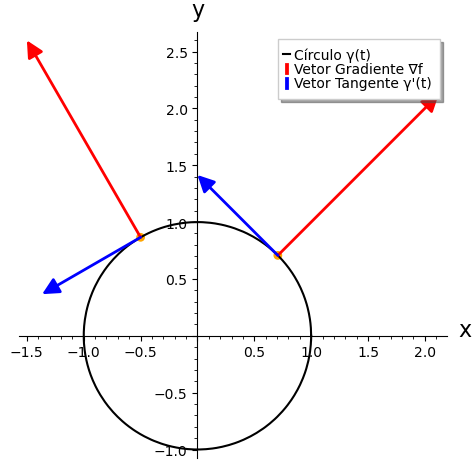
\includegraphics[width=0.25\textwidth]{imagens/av1/picture_av1_q03_item01.png}
					\captionof{figure}{Exemplo do vetor gradiente e tangente na curva $\gamma_1$}
				\end{center}
				
				\item Segunda curva de nível escolhida: $f(x,y)=2e^2$.
				Uma das curvas para essa curva de nível específica é:
				\begin{align*}
					f(x,y)=2e^2
					&\Rightarrow(x^2+y^2)\ln(x^2+y^2)=2e^2\\
					&\Rightarrow \begin{cases}x^2+y^2=e^2\\ \ln(x^2+y^2)=2\Rightarrow x^2+y^2=e^2\end{cases}
				\end{align*}
				Peguemos, então, a curva $\gamma_2$ dada pela equação $x^2+y^2=e^2$, que pode ser parametrizada como $\gamma_2(t)=(e\cos(t), e\sin(t))\Rightarrow \gamma_2'(t)=(-e\sin(t),e\cos(t))$.
				
				Agora, considere $p$ um ponto arbitrário de $\gamma_2$.
				
				\begin{align*}
					p=(x,y)\in\gamma_2
					&\Rightarrow\begin{cases}x^2+y^2=e^2\\x=e\cos(t)\\y=e\sin(t)\end{cases}\\
					&\Rightarrow\begin{cases}\nabla f(x,y)=\bigg(2x(1+\ln(e^2)), 2y(1+\ln(e^2)\bigg)=(6x, 6y)\\ \gamma_2'(t)=(-e\sin(t), e\cos(t))=(-y,x)\end{cases}\\
					&\Rightarrow\langle \nabla f(x,y),\gamma_2'(x,y)\rangle=\langle(6x,6y),(-y,x)\rangle=-6xy+6xy=0
				\end{align*}
				Assim, o gradiente do campo relativo à curva escolhida e a tangente desta mesma curva são sempre ortogonais.
				
				\begin{center}
					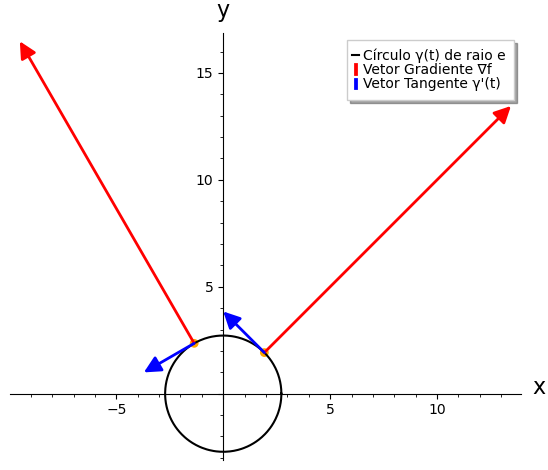
\includegraphics[width=0.25\textwidth]{imagens/av1/picture_av1_q03_item02.png}
					\captionof{figure}{Exemplo do vetor gradiente e tangente na curva $\gamma_2$}
				\end{center}
				
			\end{enumerate}
		\end{solucao}
		
		\begin{exercicio}{4}
			[1.5 ponto]
			\begin{enumerate}[label=\alph*)]
				\item Encontre a aproximação linear local $L$, no ponto $P = (0,0)$, da função
				\[
				f(x,y)=x\sin(y)
				\]
				\item Calcule o erro da aproximação de $f$ por $L$ no ponto $Q=(0.003, 0.004)$.
			\end{enumerate}
			\textit{Dica:} Reescreva a função $f\colon U\subset \mathbb{R}^2 \to \mathbb{R}$ como $graff\colon U\subset\mathbb{R}^2 \to \mathbb{R}^3$.
		\end{exercicio}
		\begin{solucao}
			Defina $graff\colon U\subset \mathbb{R}^2\to \mathbb{R}^3$, de tal forma que $graff(x,y)\coloneq (x,y,f(x,y))=(x,y,x\sin(y))$. Note que, ao calcular a aproximação linear $L$ através desse método, $L$ será a terceira coordenada da aproximação dada pela função $graff$.
			\begin{enumerate}[label=\alph*)]
				\item Calculando a sua aproximação linear $L$ através da transformação linear $J$, denominada matriz jacobiana, temos
				\[
				L=\begin{pmatrix}\nabla graff_1\\\nabla graff_2\\\nabla graff_3\end{pmatrix} =\begin{pmatrix}\tfrac{\partial x}{\partial x}&\tfrac{\partial x}{\partial y}\\\tfrac{\partial y}{\partial x} & \tfrac{\partial y}{\partial y}\\\tfrac{\partial x\sin(y)}{\partial x}&\tfrac{\partial x\sin(y)}{\partial y}\end{pmatrix}=\begin{pmatrix}1&0\\0 & 1\\\sin(y)&x\cos(y)\end{pmatrix}
				\]
				Note que, para o ponto $P=(0,0)$, temos
				\[
				J=\begin{pmatrix}1&0\\0 & 1\\\sin(0)&0\cos(0)\end{pmatrix}=\begin{pmatrix}1&0\\0 & 1\\0&0\end{pmatrix}\Rightarrow J\cdot (0,0)=(0,0,0)\Rightarrow L=0
				\]
				\item Pela definição de Frechet-diferenciável, temos que a ideia de transformação linear $J$ e o erro/resto $r_P(h)$ são definidas pela igualdade
				\[
				graff(P+h)-graff(P)=J\cdot h+r_P(h)
				\]
				Sendo $h$ um "desvio" pequeno do ponto $P$.
				
				Assim, defina $h\coloneq Q-P=(0.003,0.004)-(0,0)=(0.003,0.004)$ e temos que o vetor erro $r_P(h)$ será
				\begin{align*}
					r_P(h)
					&=graff(P+h)-graff(P)-J\cdot h\\
					&=graff(0.003,0.004)-graff(0,0)-J\cdot (0.003,0.004)\\
					&=(0.003, 0.004, 0.003\sin(0.004)) -(0,0,0)-(0.003, 0.004, 0)\\
					&=(0,0,0.003\sin(0.004))
				\end{align*}
				Logo, o erro será a terceira coordenada, dada por $E=0.003\sin(0.004)$.
			\end{enumerate}
		\end{solucao}
		
		\begin{exercicio}{5}
			[1.5 ponto] Mostre que as superfícies descritas pelas seguintes parametrizações
			\[
			X(u,v)=(u+v, u-v, 4uv), (u,v) \in \mathbb{R}^2
			\]
			\[
			Y(s,t)=(s,t,s^2-t^2), (s,t) \in \mathbb{R}^2
			\]
			têm o mesmo traço. Para um ponto $p\in S$ de sua escolha, calcule os vetores derivadas parciais para cada uma das duas parametrizações sugeridas, bem como o plano tangente $T_pS$ correspondente. Calcule os vetores normais e conclua que os planos tangentes coincidem.
		\end{exercicio}
		\begin{solucao}
			Para que as parametrizações $X$ e $Y$ tenham o mesmo traço, queremos provar que existe uma função de reparametrização/mudança de parâmetro entre ambas.
			
			Defina a função $\Phi\colon \mathbb{R}^2\to \mathbb{R}^2$, tal que $\Phi(u,v)\coloneq (u+v,u-v)$. Para ser uma função de reparametrização, devemos provar que
			\begin{itemize}
				\item $X(u,v)=Y(\Phi(u,v))$;
				\item $\Phi$ é bijetora;
				\item $\Phi$ é diferenciável e tem derivada não nula.
			\end{itemize}
			Assim, seguem as provas:
			\begin{itemize}
				\item Note que
				\begin{align*}
					Y(\Phi(u,v))
					&=Y(u+v,u-v)\\
					&=(u+v, u-v, (u+v)^2-(u-v)^2)\\
					&=(u+v,u-v,(u+v+u-v)(u+v-u+v))\\
					&=(u+v, u-v, 2u\cdot 2v)\\
					&=(u+v,u-v, 4uv)=X(u,v)
				\end{align*}
				\item Note que $\Phi$ é invertível, dado que
				\begin{align*}
					\begin{cases}\Phi_1=u+v\\\Phi_2=u-v\end{cases}
					&\Rightarrow \begin{cases}u=\tfrac{\Phi_1+\Phi_2}{2}\\v=\tfrac{\Phi_1-\Phi_2}{2}\end{cases}\\
					&\Rightarrow\Phi^{-1}(s,t)=(\tfrac{s+t}{2}, \tfrac{s-t}{2})
				\end{align*}
				Logo, $\Phi$ é bijetiva.
				\item Note que $\Phi_1$ e $\Phi_2$ são polinômios e, portanto, diferenciáveis. Calculando a derivada, temos a seguinte matriz jacobiana
				\[
				\Phi'(u,v)=\begin{pmatrix}\tfrac{\partial (u+v)}{\partial u} & \tfrac{\partial (u+v)}{\partial v}\\ \tfrac{\partial (u-v)}{\partial u} &\tfrac{\partial (u-v)}{\partial v}\end{pmatrix}=\begin{pmatrix}1&1\\1&-1\end{pmatrix}
				\]
				Assim, $\Phi$ é diferenciável e tem derivada não nula.
			\end{itemize}
			Dessa forma, concluímos que $X$ e $Y$ têm o mesmo traço.
			
			Agora, escolhido um ponto $p=(1,1,0)$, onde os parâmetros $(u,v)$ e $(s,t)$ são definidos por $p_X=(1,0)\Rightarrow p_Y=\Phi(1,0)=(1,1)$, vamos calcular os vetores derivadas parciais.
			
			Para a parametrização $X$, temos
			\begin{itemize}
				\item $\frac{\partial X(p_X)}{\partial u}=\frac{\partial (u+v,u-v,4uv)}{\partial u}=(1,1,4v)\Rightarrow\ \frac{\partial X(1,0)}{\partial u}=(1,1,0)$
				\item $\frac{\partial X(p_X)}{\partial v}=\frac{\partial (u+v,u-v,4uv)}{\partial v}=(1,-1,4u)\Rightarrow \frac{\partial X(1,0)}{\partial v}=(1,-1,4)$
			\end{itemize}
			
			Para a parametrização $Y$, temos
			\begin{itemize}
				\item $\frac{\partial Y(p_Y)}{\partial s}=\frac{\partial (s,t,s^2-t^2)}{\partial s}=(1,0,2s)\Rightarrow\ \frac{\partial Y(1,1)}{\partial s}=(1,0,2)$
				\item $\frac{\partial Y(p_Y)}{\partial t}=\frac{\partial (s,t,s^2-t^2)}{\partial t}=(0,1,-2t)\Rightarrow \frac{\partial Y(1,1)}{\partial t}=(0,1,-2)$
			\end{itemize}
			
			Para encontrar seus planos tangentes, basta encontrar os vetores normais aos planos, dados pelo produto vetorial do vetores derivadas parciais. Assim, seja $n_X$ e $n_Y$ os vetores normais dos planos tangentes às parametrizações $X$ e $Y$, respectivamente, no ponto $p$.
			\begin{itemize}
				\item $n_X=(1,1,0)\wedge(1,-1,4)=(4,-4,-2)$
				\item $n_Y=(1,0,2)\wedge(0,1,-2)=(-2,2,1)$
			\end{itemize}
			Note que $(4,-4,-2)=-2\cdot (-2,2,1)\Rightarrow n_X=-2n_Y$. Logo, os planos tangentes coincidem. Outra forma de verificar essa informação, seria calculando os planos tangentes.
			
			\begin{itemize}
				\item $n_X=(4,-4,-2)\Rightarrow T_pX\colon 4x-4y-2z=0 \Rightarrow T_pX\colon 2x-2y-z=0$
				\item $n_Y=(-2,2,1)\Rightarrow T_pX\colon -2x+2y+z=0 \Rightarrow T_pX\colon 2x-2y-z=0$
			\end{itemize}
		\end{solucao}
	
\end{document}